\documentclass[aspectratio=169]{beamer}
\usetheme{hogent}
\usecolortheme{hgwhite} % witte achtergrond, zwarte tekst
%---------- Packages ----------------------------------------------------------
\usepackage[english]{babel}      % Nederlandse taal: splitsingen, enz.
\usepackage{booktabs}          % Mooie tabellen
\usepackage{multirow,multicol} % Tabelcellen samenvoegen
\usepackage{eurosym}           % Euro symbool
%---------- Info over de presentatie ------------------------------------------
\title{The migration process and advantages of Windows Server 2019}
\subtitle{Bachelor's thesis}
\author{Jens Du Four}
\date{\today}
%==============================================================================
% Inhoud presentatie
%==============================================================================
\begin{document}
%---------- Titelpagina, inhoudstafel -----------------------------------------
{
    \setbeamertemplate{background}[imgletter]{img/background.jpg}{B}  
    \begin{frame}
    \maketitle
    \end{frame}
}

\begin{frame}
  \frametitle{Table of contents.}
  \tableofcontents
\end{frame}
%---------- Corpus ------------------------------------------------------------
\section{Introduction.}

\section{State of the art.}
\begin{frame}
\frametitle{Hybrid cloud.}  
\begin{columns}[c]
    \column{.5\textwidth}
    \colorbox{hgdarkgreen}{Types of cloud solutions}
    \begin{itemize}
        \item Private cloud
        \item Public cloud
        \item Community cloud
        \item Hybrid cloud
    \end{itemize}
    \column{.5\textwidth}

    
\end{columns}
\end{frame}
\begin{frame}
\frametitle{Security.}  
\vspace*{\fill}
    \begin{itemize}
        \item[] \colorbox{hgorange}{Windows Defender ATP}
        \item[] \colorbox{hgblue}{Security with SDN}
        \item[] \colorbox{hglightgreen}{Shieled Virtual Machines}
    \end{itemize}
\vspace*{\fill}

\end{frame}
\begin{frame}
\frametitle{Application platform.}
    \vspace*{\fill}
    \colorbox{hgdarkgreen}{Linux containers on Windows}
    \colorbox{hgpink}{Building Support for Kubernetes}
    \colorbox{hgochre}{Container improvements}
    \colorbox{hgorange}{Encrypted Networks}
    \colorbox{hgpurple}{Network performance improvements for virtual workloads}
    \colorbox{hgblue}{Low Extra Delay Background Transport}
    \colorbox{hglightgreen}{High-performance SDN gateways}
    \colorbox{hgbrown}{Persistent Memory support for Hyper-V VMs}
    \colorbox{hggrey}{New Deployment UI}
    \colorbox{hgyellow}{Windows Admin Center extension for SDN}
    \vspace*{\fill}
\end{frame}
\begin{frame}
\frametitle{Hyper-Converged Infrastructure.}  
\vspace{0.5cm}
    \begin{figure}
        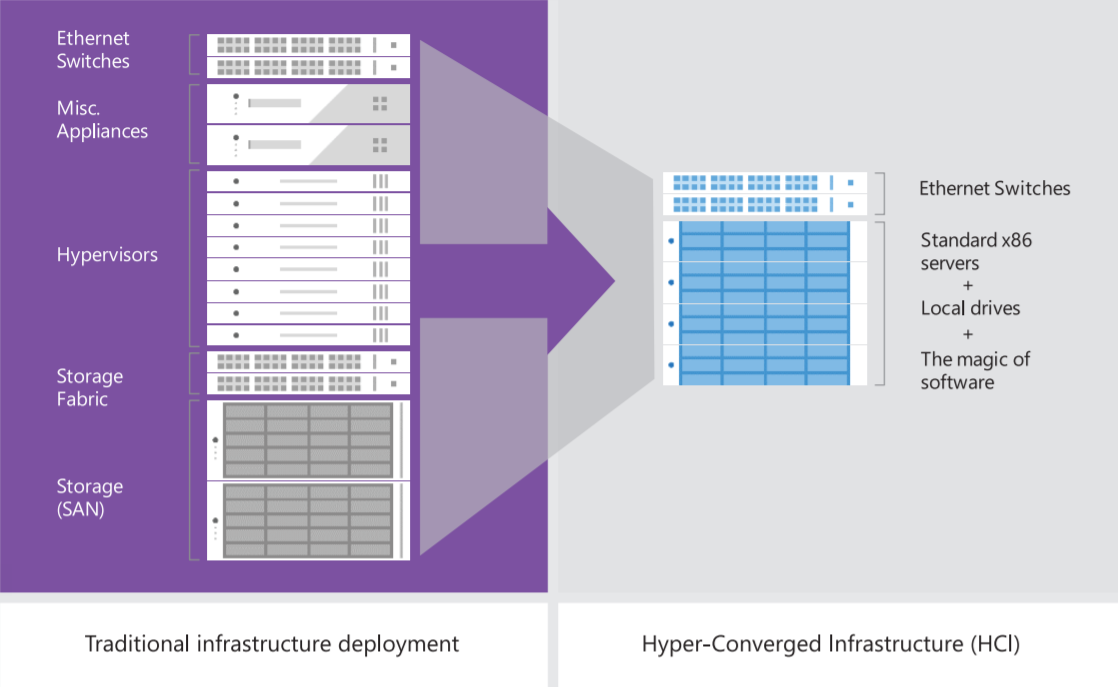
\includegraphics[height=.8\textheight]{../bachproef/img/StandVanZaken/HCI.png}
        \caption{Adapted from Woolslayer, 2018.}
    \end{figure}
\end{frame}

\section{Methodology.}
\begin{frame}
\frametitle{In-place upgrade.}  
\vspace{0.5cm}
\begin{figure}
    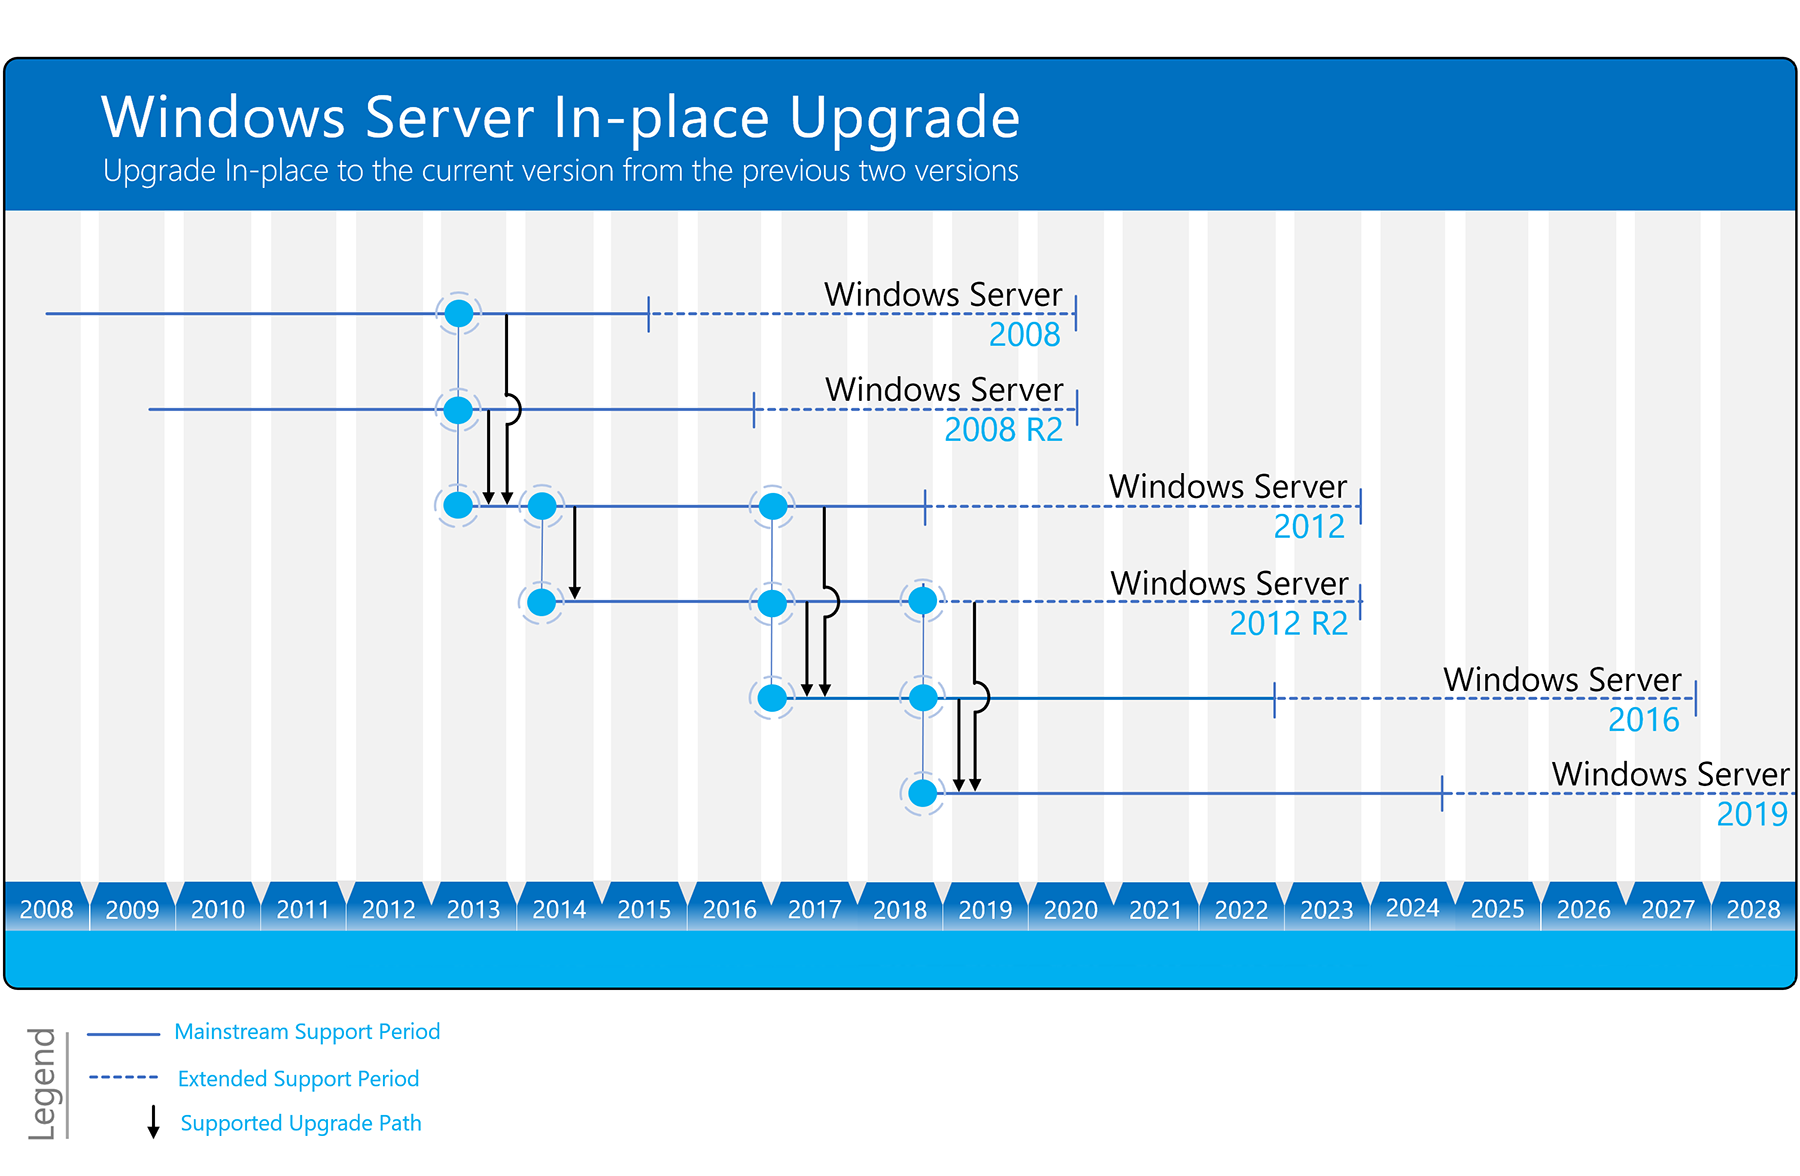
\includegraphics[height=.8\textheight]{img/upgrade}
    \caption{Adapted from Plett, 2018.}
\end{figure}
\end{frame}
\begin{frame}
\frametitle{Side-by-side migration.}  
\vspace{0.5cm}
\begin{figure}
    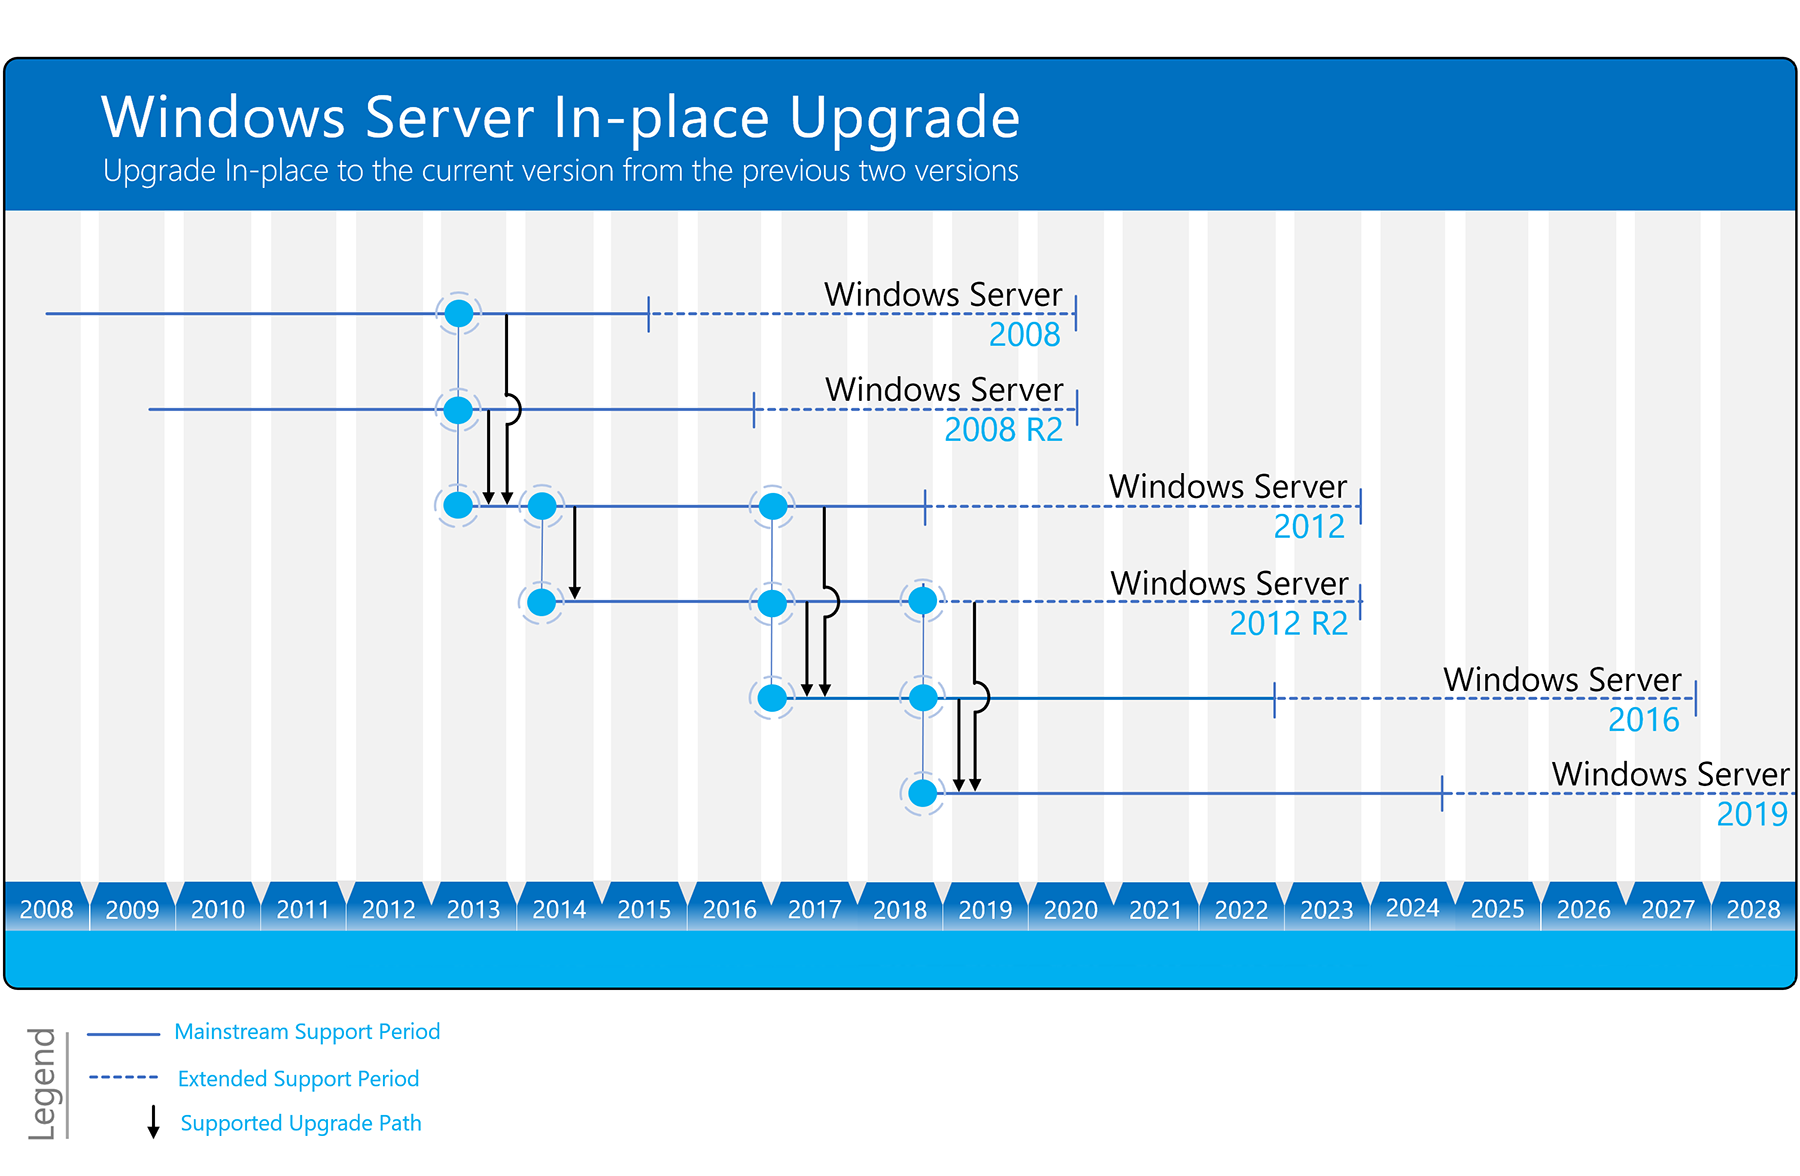
\includegraphics[height=.8\textheight]{img/upgrade}
    \caption{Adapted from Plett, 2018.}
\end{figure}
\end{frame}
\begin{frame}
\frametitle{Base container images.}  
  \begin{table}
    \begin{tabular}{llll}
        \toprule
        & \textbf{Windows} & \textbf{Server Core} & \textbf{Nano Server} \\
        \midrule
       Version 1809 & $9.9$ GB & $4.28$ GB              & $347$ MB \\
        \midrule
        Version 1709 & & $6.47$ GB              & $339$ MB \\
        \bottomrule
    \end{tabular}
    \caption{Base container image size}
\end{table}
\end{frame}
\begin{frame}
\frametitle{Base container images.}  
\vspace{0.5cm}
\begin{figure}
    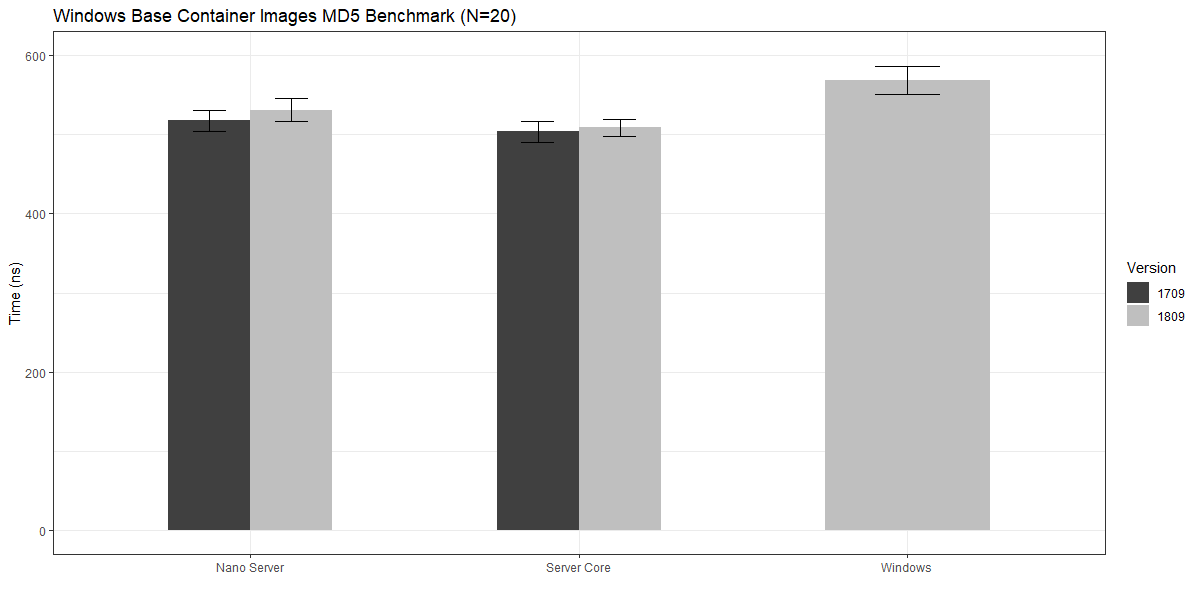
\includegraphics[height=.8\textheight]{../bachproef/img/Methodologie/Containers1.png}
\end{figure}
\end{frame}

\section{Future vision.}
\begin{frame}
\frametitle{Future vision.}  
\vspace{0.5cm}
\begin{figure}
    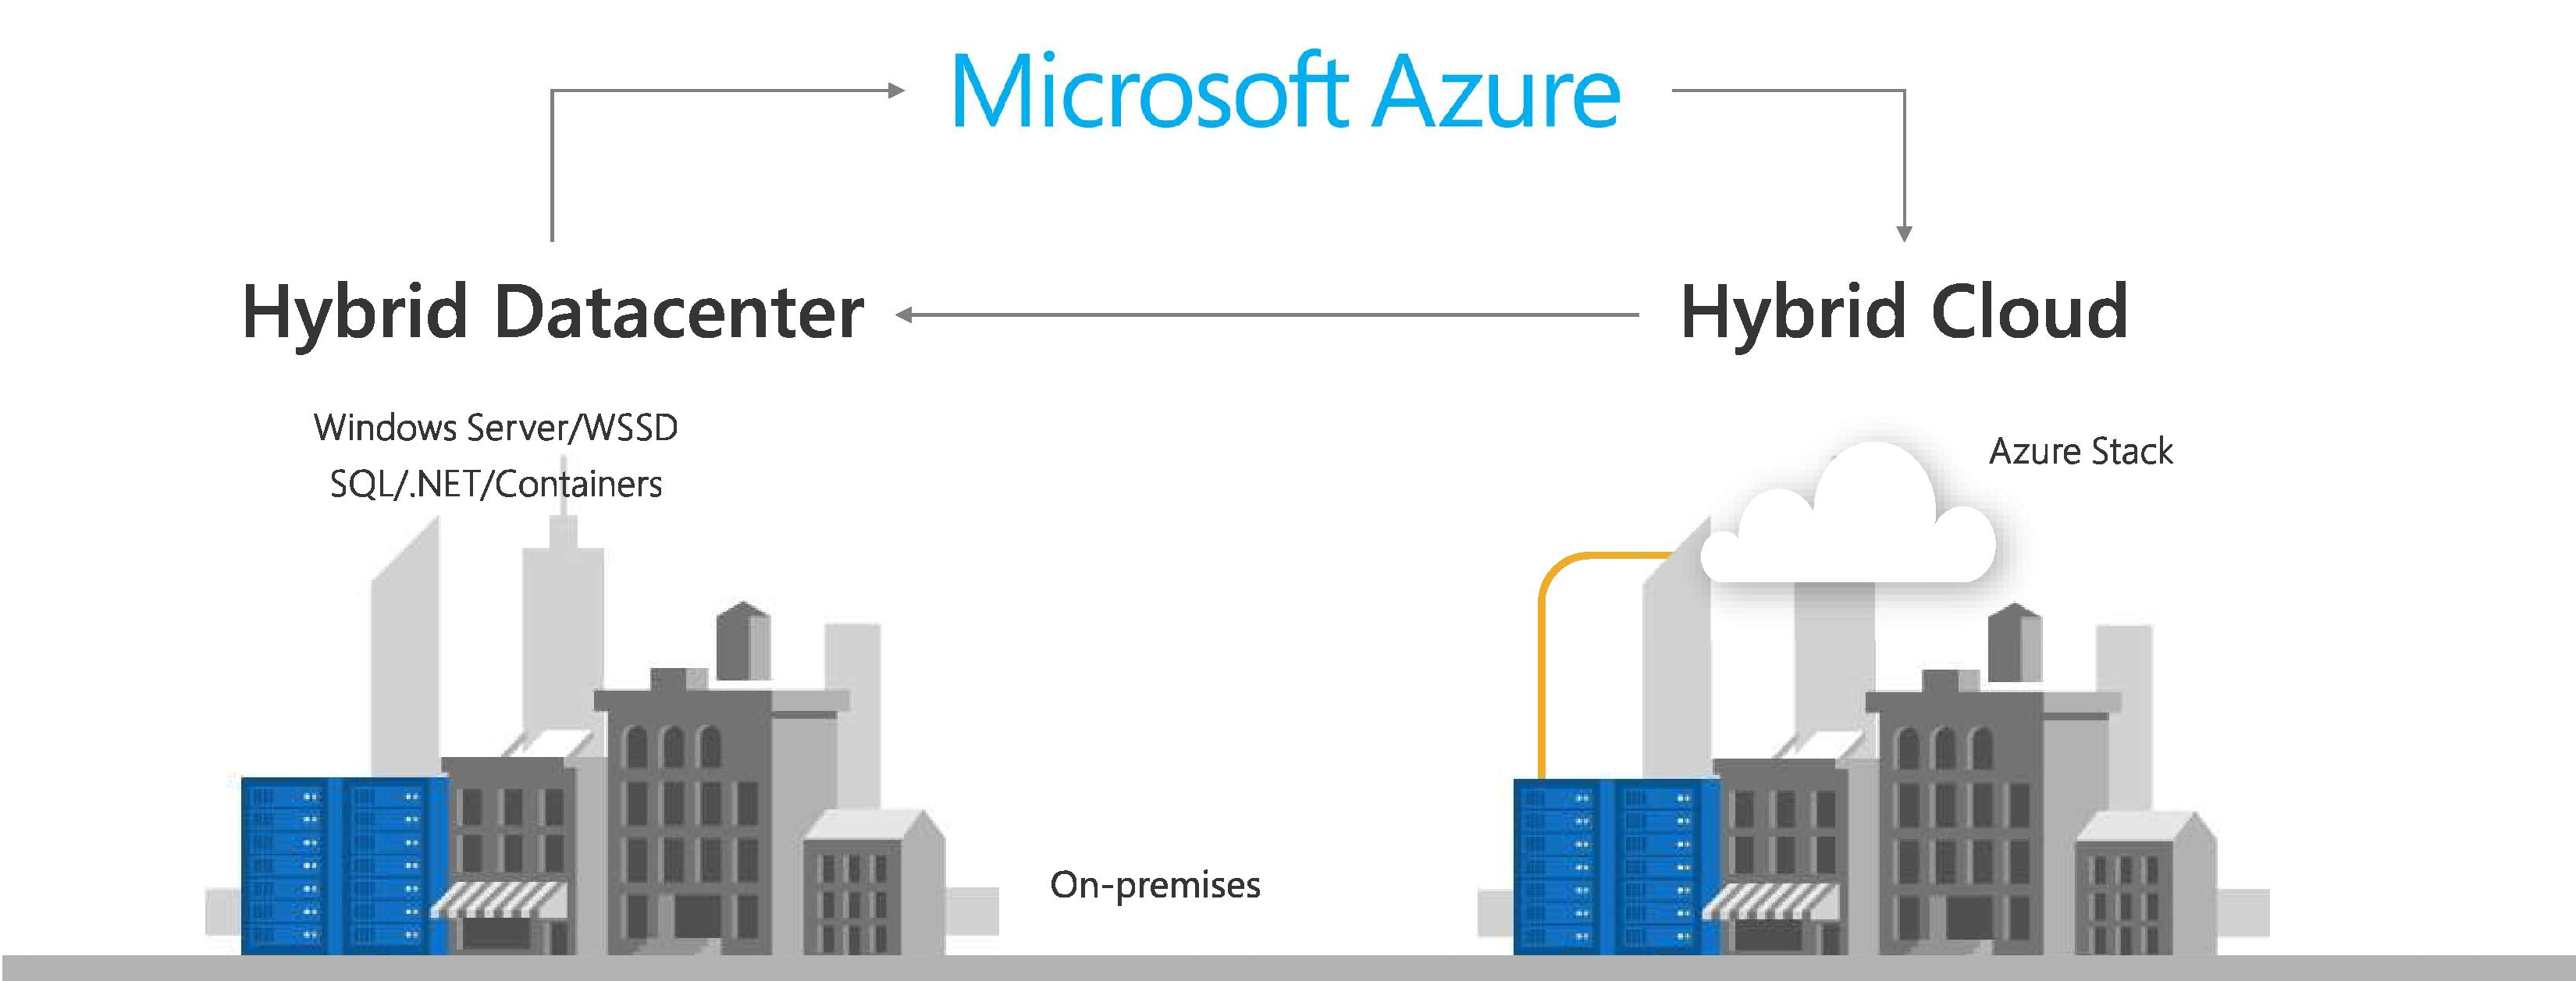
\includegraphics[height=.7\textheight]{../bachproef/img/Toekomstvisie/Azure1.png}
    \caption{Adapted from A. Singh and Shah, 2019}
\end{figure}
\end{frame}
\section{Conclusion.}

\section{Questions?}

\end{document}
